\chapter{Introduction}
\label{chap:1}

Neuroscientists, to diagnose a psychiatric disorder, use symptom scores from clinical interviews. For a definitive validation, could be useful to study the interactions between brain regions, in order to see the different behaviours of these interactions in a brain of Typical Developed people and people with disorders. This could be seen through Magnetic Resonance Imaging (MRI), in particular functional MRI (fMRI). The neuroimaging data produced are then pre-processed and transformed in structures that an algorithm can study, in our cases graphs, matrices and time series. From the study of these interactions the important thing that we need to implement is the classification of the brain representation, meaning that each method taken in consideration in this work has the aim to implement a classification that says whether the brain that I give to it is affected by a disorder. This is called brain classification. 

The studies taken in consideration, other than in techniques, differs also in the data that have in input. The inputs could be graphs, matrices, time series and even images. This work is focused on methods that take in input graphs, even in matrix representation. Many methods have been implemented for graph classification. They are important tools that can be applied in many fields and subjects. In our particular field, graph classification of brain networks, becomes important to take in account the structure of the graph, because there could be many brain regions that characterize a specific psychiatric disorder. We will see how in some methods are also studied those regions to identify the once that have different interactions in people with disorders, even if the described experiments of this works are concentrated on the simple classification of brain networks. 

This thesis contains an explanation of the basics with which the study works, then a description of several methods on this subject and then experiments with some of these methods that more represent our field. 

This work was performed during a research internship at ISI Foundation
under the supervision of Dr. Francesco Bonchi.

\section{Outline}
The thesis is organized as follows:

\begin{itemize}
	\item In the current chapter there is an explanation of some basics related to this work.
	\item Chapter \ref{chap:2} contains the classification of the several methods taken in account, so, an overview of the macro-classes of all the implemented techniques to do \emph{graph} and \emph{brain classification}. 
	Then, for each method, there is an explanation of the main characteristics.
	\item Chapter \ref{chap:3} contains the experimental part. Are described the set-up of the experiments, like the datasets and the kind of classification, the results of the experiments and a discussion of the results.
	\item Chapter \ref{chap:4} contains comments about the use of each method and possible future works. 
\end{itemize}

\section{Background}
To understand better all the methods, we should do some explanation of what we will encounter during the lecture. The main arguments we should consider are \textbf{Graphs}, \textbf{Classification} and \textbf{Connectomes}.

\paragraph{Graphs} \
\\
There are many subjects in which graphs are used, and consequently many definitions. In mathematics, a graph is a structured set of objects that, in pairs, could have a relation between themselves. Each object is called a \textit{vertex}, and each relation between a pair of vertices is called an \textit{edge}. So, a graph $ G(V,E) $ is a pair where $ V $ are the vertices and $ E $ are the edges. Graphs are represented in diagram form, where vertices are in circle form and edges are lines that join pairs of vertices with a relation.
\begin{figure}[htbp]
	\centering
	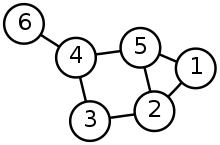
\includegraphics[scale=0.5]{Immagini/220px-6n-graf.svg.png}
	\caption{\label{fig:diagram}}
\end{figure}

Graph could be \textit{directed} or \textit{undirected}. In a direct graph, edges have an orientation, the links between vertices can be represented by arrows going from one vertex to the other. In an edge $ (x,y) $ directed from $ x $ to $ y $, the vertices are called respectively \textit{tail} and \textit{head} of the edge.
\begin{figure}[htbp]
	\centering
	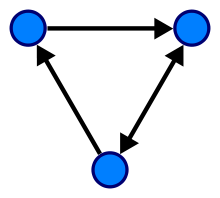
\includegraphics[scale=0.5]{Immagini/220px-Directed.svg.png}
	\caption{\label{fig:diagram2}}
\end{figure}

Graphs can be represented by matrices, the matrix representations in which we are interested for this thesis are \textbf{Adjacency matrix} and/or \textbf{Connectivity matrix}. 

An \textbf{Adjacency matrix} is a square matrix that represents if there is an edge between two vertices. In particular in an unweighted graph with a vertex set $ U=\{u_{1}, ..., u_{n}\} $ the Adjacency matrix $ A $ is an $ n \x n $ matrix in which its element $ A_{ij} $ is 1 if there is an edge between the vertices $ u_{i} $ and $ u_{j} $. If the graph is weighted the values in the matrix are not 1s and 0s, but depends on the weight of each edge. Also, if the graph is undirected the Adjacency matrix is symmetric.

The Adjacency matrix sometimes is called \textbf{Connectivity matrix}.

\paragraph{Classification}\
\\
In machine learning, \emph{Classification} is a supervised learning approach in which an algorithm is trained, with some given data, to classify new observations. It is a process. 

First we have some data, of which we already know the belonging class, called \emph{labelled} data. We could have two classes, in which case we will have a \emph{binary classification}, or multiple classes, so \emph{multi-class classification}. Our labelled data are given to the classification model, starting the \textbf{training} of the model.

Once trained the classificator, we can give to it new data that we want to classify. This is called the \textbf{prediction}. Finished the prediction we can evaluate our model through some scores, the main one in our case is the \textbf{accuracy}, that calculates the percentage of how many predictions of our classifier are right. 

\paragraph{Connectomes}\
\\
The \textbf{connectome} is the connection matrix of the human brain \cite{connectome}. From the anatomic point of view, the connectome is defined by all the axonal origins, terminations and trajectories of all the brain neurons, through the brain regions. This means, the connectivity of neural pathways in the brain. 

Being able to have a representation of the human brain allows us to understand fundamental cognitive operations, brain activities, conditional structure-function models of the brain, so, consequently, to understand and detect brain deceases. From this powerful tool, we can see how brain physiology is correlated to abilities and behaviours, underlying mental anomalies and pathology. This is fundamental to develop treatments ad hoc for each pathology and case. 

Other fields, that we do not cover here, but that are very interesting, concern the memories (in fact neuroscientists believe that our memories are stored in the synapses between neurons) and the preservation of the brain (being able to recover the structure and connections of it).
https://www.brainpreservation.org/content-2/connectome/

In the following image we can see an example of a connectome.

\begin{figure}[htbp]
	\centering
	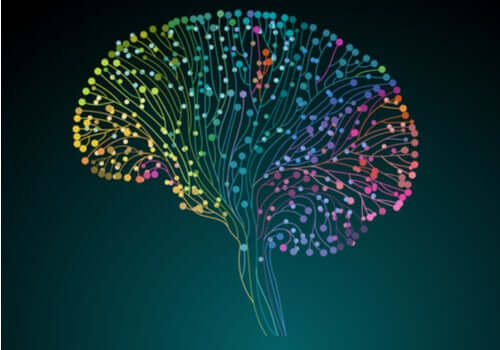
\includegraphics[scale=0.3]{Immagini/cervello-connessioni-neuroni-colorate.jpg}
	\caption{\label{fig:diagram3}}
\end{figure}



\section{Related works}\
\\
Here we concentrate the study of connectomes in graph form. This means that the fMRI of a brain, elaborated in a connectome, is then transformed in graph form, and the graph is studied in matrix form. The graph have as nodes the brain regions, and as edges the connections between them. It follows that the matrix is an \emph{Adjacency matrix}, in which the values represent the degree of connections between the regions, and each row and each column is a node of the graph, a so called \emph{Region of interest} (\textbf{ROI}).
\begin{figure}[htbp]
	\centering
	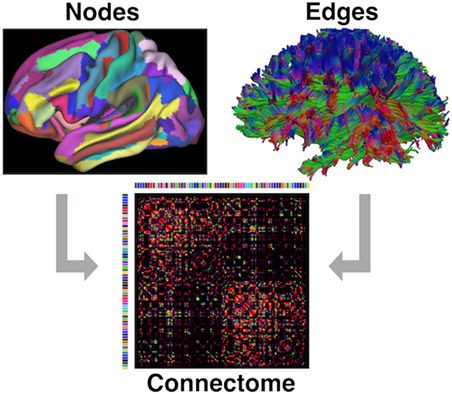
\includegraphics[scale=1]{Immagini/nbm3752-toc-0001-m.jpg}
	\caption{\label{fig:diagram4}}
\end{figure}

\paragraph{Graph Classification}\
\\
The technique that studies the classification of graphs is called \textbf{Graph Classification}. The basic definition of graph classification is \cite{10.1145/3219819.3219980}: given a set of graphs $\mathcal{B}=\left\{\left(\mathcal{G}_{1}, \ell_{1}\right),\left(\mathcal{G}_{2}, \ell_{2}\right), \cdots,\left(\mathcal{G}_{n}, \ell_{n}\right)\right\}$ the aim is to learn a function $f: \mathbf{G} \rightarrow \mathcal{L}$, where $\mathbf{G}$ is the input space of graphs, and $\mathcal{L}$ is the set of graph labels. Each graph $\mathcal{G}_{i}=\left(\mathbf{A}_{\mathcal{G}_{i}}, \mathbf{B}_{\mathcal{G}_{i}}\right)$ has an adjacency matrix $\mathbf{A}_{\mathcal{G}_{i}} \in\{0,1\}^{N_{i} \times N_{i}}$ and an attribute matrix $\mathbf{B}_{\mathcal{G}_{i}} \in\ \mathbf{R}^{N_{i} \times N_{i}}$, where ${N}_{i}$ is the number of nodes of the $i$-graph and $B$ is the number of attributes. Each graph has also a corresponding label $l_{i}$. 	

The usual strategy to study graphs is to calculate graph statistics on the entire graph. A popular technique is to count the occurrences of various \textit{subgraphs} on a graph, called graphlet kernel \cite{pmlr-v5-shervashidze09a}. Then there is the \textit{Morgan algorithm} \cite{Rogers2010ECFP} that consists in an iterative process, that updates the attributes vector of each node by hashing a concatenation of all the attributes of in the node's local neighbourhood. Then from the final attributes of all the nodes in the graph is computed the graph feature. Recently, learning data-driven graph features \cite{NIPS2015_f9be311e} is becoming more important. This means that given a dataset, the task-relevant features are learned automatically from the graphs. Once we extract these features, independently of which method we would like to use, we use them for the classification.
Another method that we can mention is all the literature that regards \textit{Graph Neural Networks} (GNN), a deep learning technique. To build a GNN we need to find out the graph structure, the graph type and its scale, then we should define the loss function, depending on the task, and then we are ready to build a model using computational model \cite{ZHOU202057}. 

These methods brings us to the field of our interest, \textbf{Brain Classification}. For Brain Classification have been used the previous graph classification techniques, adapted for a more suitable result. In the next chapter we will discuss various methods that inspired this work.